\chapter{Test dei metodi di spam detection}
\lstset{basicstyle=\small\ttfamily,keywordstyle=\color{black}\bfseries,commentstyle=\color{darkgray},stringstyle=\color{black},showstringspaces=true} 
Nei capitoli precendenti sono stati illustrati vari metodi che di spam detection classificati basandosi sui segnali in ingresso che essi hanno bisogno per poter identificare le pagine web; quindi si hanno tre classi: metodi basati sul contenuto, metodi basati sul grafo e metodi che utilizzano segnali diversi dai primi due. Tra questi metodi ne sono stati presi in esame due: \textit{Trustrank} e \textit{Anti-trust rank}. 

Si è scelto, quindi, di valutare l'efficacia di due  algoritmi \textit{linked base} (\textit{Trustrank} e \textit{Anti-trust rank}) se essi operassero in modo online. Più precisamente i vari test consistono nel verificare quanto questi due algoritmi di tipo offline riescano ad approssimare il loro comportamento se li facessimo operare in modo online ovvero durante la fase di crawling. Le domande che ci poniamo eseguendo questi test su i due algoritmi di spam dection offline (\textit{Trustrank} e \textit{Anti-trus rank}) sono:
\begin{itemize}
 \item possono questi algoritmi essere in grado di operare in modalità online?
 \item durante l'esecuzione in modalità online, quanto riescono ad approssimare il loro comportamento offline?
 \item è conveniente utilizzare questi algoritmi in modalità online?
\end{itemize}

E' doveroso specificare che un algoritmo di spam detection lavora offline se questo viene eseguito dopo l'attività di crawling (e quindi dopo che si ha a disposizione l'intero grafo ottenuto dai collegamenti tra le pagine), mentre un algoritmo di spam detection lavora online se questo viene eseguito durante il processo di crawling e quindi riesce a determinare all'istante se una pagina deve essere considerata spam o non spam. Dal momento che si è scelto di esaminare degli algoritmi \textit{linked base}, e sapendo che questi formulano delle conclusioni sulla natura delle pagine (ovvero se sono spam o non spam) esaminando la struttura dell'intero grafo, è interessante notare come questi si comportino se il grafo su cui fare le valutazioni è incompleto.
%altre considerazioni

Il capitolo è diviso nel seguente modo: nella prima parte verrà illustrato come è stato scelto di simulare il crawler per poter eseguire gli algoritmi offline duratne la fase di crawling; nella seconda parte verrà spiegato come sono stati implementati i test; infine verrano illustrati tutti i test.

\section{Simulazione del crawler}
Per simulare il comportamento di crawler, e quindi eseguire gli algoritmi di \textit{Trustrank} e \textit{Anti-trust rank}, abbiamo implementato una semplice visita sul grafo in ampiezza ovvero una BFS \cite{bfsCormen} (Breadth-First Search). La visita in ampiezza dato un grafo \(G=(V,E)\), dove \(V\) è l'insieme dei vertici del grafo ed \(E\) l'insieme degli archi del grafo, e un vertice \(s\) da cui far partire la visita, scopre tutti i vertici che sono raggiungibili da \(s\). La visita in ampiezza scopre tutti i vertici che si trovano a distanza \(f\) dal vertice di partenza e successivamente scopre i vertici che si trovano a una distanza successiva \(f+1\). In sostanza dato il nodo di partenza \(s\), la visita in ampiezza, scopre tutti i nodi vicini al nodo \(s\) e successivamente per ogni nodo vicino scoperto trova i vicini che non sono ancora stati visitati; questo processo viene iterato finche tutti i nodi del grafo raggiungibili da \(s\) sono visitati. \\
Quindi anziche implementarci l'algoritmo BFS abbiamo utilizzato l'implementazione definita nel framework WebGraph. In particolare è stata utilizzata la classe ``ParallelBreadthFirstVisit'' che esegue una visita in ampiezza utilizzando il parallelismo derivato dai processori multicore.

\section{I test}
Come gia introdotto lo scopo dei test consiste che dato un algoritmo di spam detection che opera in modo offline valutare le sue prestazioni se operasse in modo online. Oltre tutto abbiamo scelto due algoritmi \textit{linked base} quali \textit{Trustrank} e \textit{Anti-trust rank} questo significa che l'algoritmo opererà su un grafo del web incompleto, all'inizio del crawling, fino ad arrivare ad operare sull'intero grafo alla fine del crawling.

\begin{figure}
\centering
 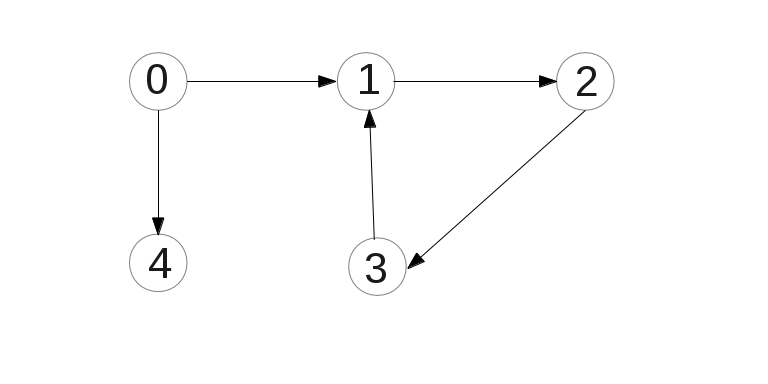
\includegraphics{immagini/test/grafoComp}
 \caption{Esempio di grafo}
 \label{fig:grafoComp}
\end{figure}

Quasi tutti i test seguono uno stesso schema; viene eseguito \textit{Trustrank} (e \textit{Anti-trust rank}) sul grafo completo, e lo indicheremo con \(t\) (\textit{Anti-trust rank} sarà indicato con \(a\)), successivamente viene eseguita la BFS (ovvero la visita in ampiezza) con nodo sorgente \(s\) e quindi si ricava la coda \(q\) dei nodi visitati a partire da \(s\); dopo di che si calcola \textit{Trustrank} (e \textit{Anti-trust rank}) sul grafo ricavati lungo la visita in ampiezza formato, quindi, da un sottoinsieme di nodi \(q\), il risultato lo indicheremo con \(\hat{t}_i\) (\textit{Anti-trust rank} sarà indicato con \(\hat{a}_i\)) dove \(i\) è il numero di nodi presi in considerazione dalla coda \(q\). Questo processo viene iterato incrementando sempre di più l'intervallo \(i\) finché non si arriva alla fine della coda \(q\) dei nodi visitati partendo dal nodo \(s\). Dopo aver calcolato \(t\) e \(\hat{t}_i\) sono due vettori si possono valutare tramite la Tau di Kendall e indicheremo con \(\tau(t,\hat{
t}_i)\) la Tau di Kendall per \(t\) e \(\hat{t}_i\)  (e quindi \(\tau(a,\hat{a}_i)\) sarà la Tau di Kendall per \(a\) e \(\hat{a}_i\)). Ad esempio in figura \ref{fig:grafoComp} è rappresentato il grafo completo su cui verra calolato \(t\) e \(a\) mentre in figura \ref{fig:grafo3} è rappresentato il grafo ricavato dalla BFS eseguita sul grafo precedente partendo dal nodo 1; se si considerano tutti i nodi lungo la visita il vettore di \textit{trustrank} sarà \(\hat{t}_3\) mentre quello di \textit{anti-trust rank} sara \(\hat{a}_3\)..

 \begin{figure}
\centering
 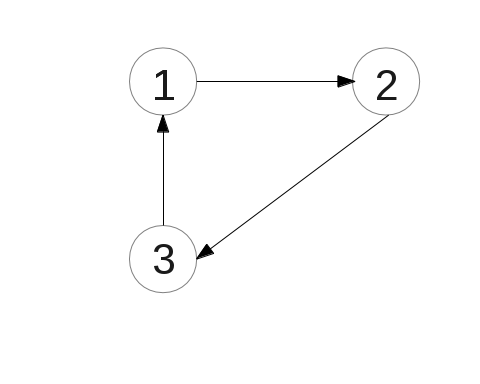
\includegraphics{immagini/test/grafo3}
 \caption{Esempio di grafo ricavato tramite una BFS a partire dal nodo 1 del grafo in figura \ref{fig:grafoComp}.}
 \label{fig:grafo3}
\end{figure}
A ogni indice del  vettore di \textit{Trustrank} \(t\) e del vettore di \textit{Anti-trust rank} \(a\) corrisponderà un nodo è il valore del vettore per un dato indice indica il valore di \textit{Trustrank} e \textit{Anti-trust rank} del nodo del grafo. In figura \ref{fig:tVettore} è illustrato un esempio del vettore di \textit{trustrank} calcolato sull'intero grafo e in figura \ref{fig:aVettore} è illustrato un esempio del vettore di \textit{anti-trust rank} calcolato sull'intero grafo. 
Nell'esempio in figura \ref{fig:tVettore} si nota che il vettore \(t\) di \textit{trustrank} ha lunghezza 5, quindi il grafo sarà composto da 5 nodi dove ad ogni nodo è associato il valore di \textit{trustrank}. Le stesse considerazioni valgono per l'esempio in figura \ref{fig:aVettore} dove il vettore di \textit{anti-trust rank} è ha lunghezza 5 e quindi l'algoritmo opererà su un grafo composto da 5 nodi.

\begin{figure}
\centering
 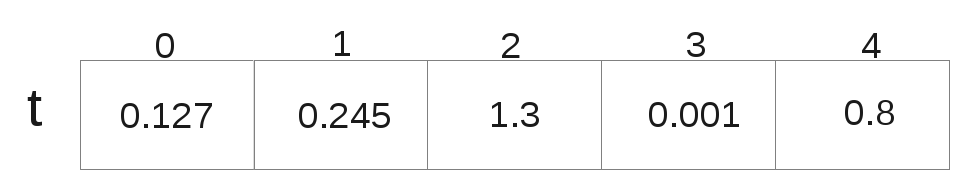
\includegraphics{immagini/test/trustVettore}
 \caption{Esempio del vettore di trustrank calcolato sull'intero grafo}
 \label{fig:tVettore}
\end{figure}
\begin{figure}
\centering
 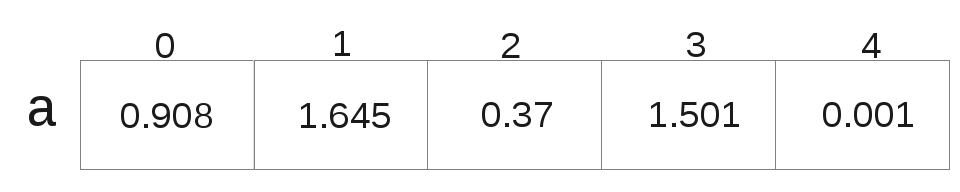
\includegraphics{immagini/test/immagineAntiTrust}
 \caption{Esempio del vettore di anti-trust rank calcolato sull'intero grafo}
 \label{fig:aVettore}
\end{figure}

A differenza dei vettori \(t\) e \(a\) (\textit{trustrank} eseguito sull'intero grafo e \textit{anti-trust rank} sull'intero grafo) , dove ad ogni indice (cioè ad ogni nodo) è associato un valore di \textit{trustrank} e \textit{anti-trust rank} , i vettori \(\hat{t}_i\) e \(\hat{a}_i\) non avranno per ogni indice un valore associato. Più precisamente, sapendo che \(\hat{t}_i\) e \(\hat{a}_i\) sono calcolati durante l'esecuzione di una BFS allora a ogni passo ci saranno ancora dei nodi da visitare per cui non è possibile calcolare i valori di \textit{trustrank} e \textit{anti-trust rank}, perciò con l'avanzamento della visita in ampieza sempre più nodi avranno associato un valore di \textit{trustrank} e \textit{anti-trust rank}. Vale quindi che \(\hat{t}_{i+1}\) avrà molti più nodi per cui è stato calcolato \textit{trustrank} rispetto a \(\hat{t}_i\) (lo stesso comportamento si riscontra per \textit{anti-trust rank}). Inoltre non è detto che dopo aver terminato la visita in ampiezza, partendo da un nodo \(s\),
 si sia visitato tutto il grafo (ovvero che \(s\) può raggiungere tutti i nodi del grafo) perciò in questo caso \(\hat{t}_i\) e \(\hat{a}_i\) avranno un numero minore di nodi per cui è calcolato \textit{trustrank} e \textit{anti-trust rank} rispetto a \(t\) e \(a\).\\
Dal momento che la Tau di Kendall tra due vettori, per essere eseguita, richiede che i due vettori abbiano la stessa lunghezza allora bisogna gestire i casi in cui i nodi del grafo temporaneo (ottenuto ad ogni intervallo di nodi visitato tramite la visita in ampiezza) non abbiano associato un valore. Per gestire tale problema si è scelto di considereare i soli nodi compresi nel grafo temporaneo. Ad esempio in figura \ref{fig:tBFSmodoB} viene illustrato il caso in cui eseguendo la BFS dal nodo 1, i nodi 0 e 4 rimangano senza aver assegnato un valore di \textit{trustrank}. Quindi gli indici 0 e 4 del vettore \(t\) non sono inclusi nel vettore \(\hat{t}_3\) questo implica che ci deve essere una corrispondenza tra gli indice del vettore \(t\) e quelli del vettore \(\hat{t}_3\) (in figura \ref{fig:tBFSmodoB} l'indice 0 del vettore \(\hat{t}_3\) corrisponde all'indice 1 del vettore \(t\), l'indice 1 al indice 2 ed infine l'indice 2 all'indice 3).  Si inoltre nota che il vettore \(\hat{t}_3\) ha lunghezza inferiore 
al vettore \(t\). Inoltre il calcolo della Tau di Kendall sara tra il vettore \(t\) formato dai soli indici compresi nel vettore \(\hat{t}_i\) e dal vettore \(\hat{t}_i\). Quindi  nella valutazione  il vettore \(t\) dovra essere ristretto alla lunghezza del vettore \(\hat{t}_i\) e quindi dovranno essere eliminati gli indici del vettore \(t\) che non sono inclusi nel vettore \(\hat{t}_i\).
\begin{figure}
\centering
 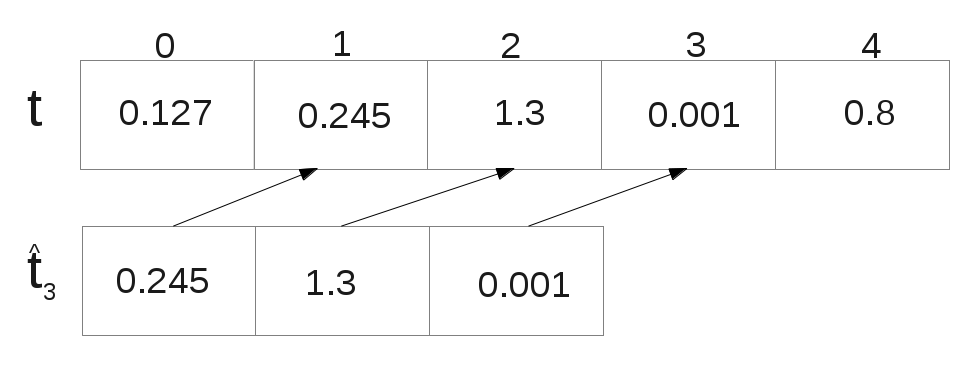
\includegraphics{immagini/test/tBFSmodoB}
 \caption{Esempio del vettore di trustrank calcolato su una porzione di grafo.}
 \label{fig:tBFSmodoB}
\end{figure}
Un altro metodo che può essere utilizzato è quello di assegnare ad ogni indice dei vettori \(\hat{t}_i\) e \(\hat{a}_i\) non ancora visitati il valore 0.0. Ad esempio prendendo in considerazione il grafo in figura \ref{fig:grafoComp} e ipotizzando di eseguire una BFS a partire dal nodo 1 e di aver visitato i nodi 2 e 3 quindi se calcoliamo \textit{trustrank} e \textit{anti-trust rank} sul sottografo ricavato dai nodi visitati, i nodi 0 e 4 avranno associato i valori 0.0 (usando il metodo \textit{Modo\_A}), tale esempio è illustrato in figura \ref{fig:tBFSmodoA} e in figura \ref{fig:aBFSmodoA}. Questa metodo però è poco significativo in quanto vengono introdotti dei valori non veritieri che producono rumore, e quindi non verrà preso in considerazione.
\begin{figure}
\centering
 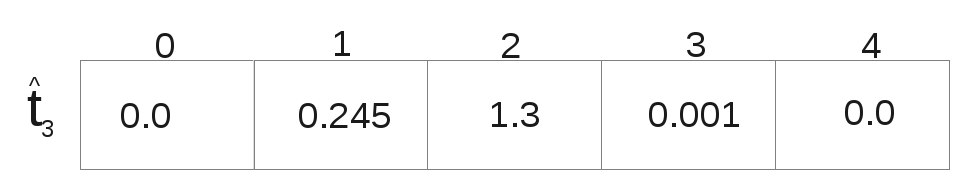
\includegraphics{immagini/test/tBFSmodoA}
 \caption{Esempio del vettore di trustrank calcolato su una porzione di grafo a cui viene assegnato il valore 0.0 ai nodi non visitati.}
 \label{fig:tBFSmodoA}
\end{figure}
\begin{figure}
\centering
 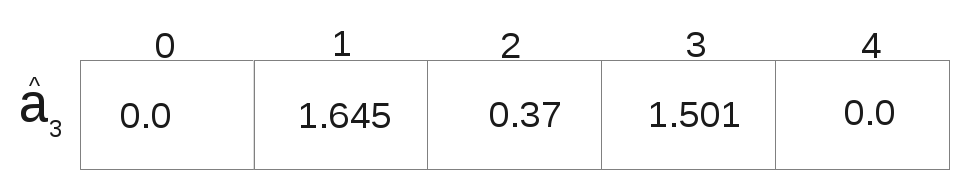
\includegraphics{immagini/test/aBFSmodoA}
 \caption{Esempio del vettore di anti-trust rank calcolato su una porzione di grafo a cui viene assegnato il valore 0.0 ai nodi non visitati.}
 \label{fig:aBFSmodoA}
\end{figure}

I test saranno, quindi, cosi strutturari:
\begin{itemize}
 \item Test numero 1. Si confronta \textit{trustrank} sul grafo completo con \textit{trustrank} calcolato su una porzione di grafo. Lo stesso si fa per \textit{anti-trust ran}.
 \item Test numero 2. Si confrontano i solo nodi etichettati spam del vettore di  \textit{trustrank} sul grafo completo con  i soli nodi etichettati spam del vettore di \textit{trustrank} calcolato su una porzione di grafo. Nel caso di \textit{anti-trust rank} si  confrontano i nodi etichettati come non spam.
 \item Test numero 3. Si calcola \textit{trustrank} sul grafo completo ottenuto eseguendo la visita partendo da un nodo \(s\) e si confronta con \textit{trustrank} eseguito a ogni passo delle visita ma si imposta un seedset diverso formato dagli ultimi \(n\) nodi della vista. Viene applicato lo stesso metodo per \textit{anti-trust rank}.
 \item Test numero 4. Si esegue la BFS a partire dal nodo \(s\) e per ogni passo si calola la media dei valori di \textit{trustrank} dei soli nodi che sappiamo essere non spam e la media dei valori di \textit{Trustrank} dei soli nodi spam. Quindi si calcola la differenza tra le due medie. Lo stesso metodo verrà applicato per l'analisi dell'algoritmo di \textit{anti-trust rank}.
 \end{itemize}
 
\section{Test 1}
 Questo test calcola la distanza, tramite della Tau di Kendall denominata \(T_t\), tra il vettore \(t\) di \textit{trustrank} ricavato sull'intero grafo e il vettore \(\hat{t}_i\) di \textit{trustrank} calcolato sul grafo ricavato dai nodi visitati lungo una visita in ampiezza con nodo sorgente \(s\). Inoltre viene eseguto lo stesso procedimento per quanto riguarda \textit{anti-trust rank} ovvero si calcolano le distanze, sempre utlizzando una Tau di Kendall che denomineremo \(T_a\),  tra il vettore di \(a\) di \textit{anti-trust rank} ottenuto dal grafo completo e il vettore \(\hat{a}_i\)  caloato sul grafo ricavato dai nodi visitati lungo  un visita in ampiezza con nodo sorgente \(s\). Dal dataset sono impostati come nodo sorgente della BFS due nodi: il nodo 62 etichettato come non spam e il nodo 112 etichettato come spam. Inoltre per il calcolo di \textit{trustrank} sull'intero grafo viene utilizzato come seedset l'insieme di pagine del dataset WEBSPAM-UK2007 etichettate come non spam mentre per il calcolo di \textit{trustrank} sul grafo ottenuto dai nodi visitati durante la BFS il seedset sarà formato dalle pagine visitate che sono etichettate come non spam nel dataset WEBSPAM-UK2007. Per il calolo di \textit{anti-trust rank} sull'intero grafo, invece, il seedset sarà composto dalle pagine etichettate come spam nel dataset WEBSPAM-UK2007 mentre il seedset di \textit{anti-trust rank} calcolato sul grafo ottenuto dai nodi visitati dalla BFS sarà formato dai soli nodi visitati che sono etichettati come spam.

In figura \ref{fig:test1trustModoB62} e in figura \ref{fig:test1trustModoB112} sono rappresentati rispettivamente i grafici delle Tau di Kendall \(T_{t62}\) e \(T_{t112}\), per il cacolo delle distanze tra il vettore \(t\) calcolato sull'intero grafo e il vettore \(\hat{t}_i\) calcolato sul grafo ottenuto dai nodi visitati lungo una visita in ampiezza con nodo sorgente nel primo caso 62 e nel secondo con nodo sorgente 112.  Sull'asse delle ascisse è rappresentato il numero di nodi che sono stati visitati attraverso la BFS e quindi il numero di nodi del grafo su cui viene calcolato \(\hat{t}_i\) dove \(i\) è appunto il numero di nodi presi in considerazione, mentre sull'asse delle ordinate è rappresentato il valore della Tau di Kendall tra il vettore \(t\) e \(\hat{t}_i\).\\
I due grafici sono molto simili è quindi il calcolo di \(\hat{t}_i\) non dipende dal nodo da cui sorgente della visita in ampiezza. Il valore di Tau di Kendall uguale ad 1 si ha quando la BFS ha visitato solamente il nodo di partenza, quindi  il vettore \(t\) avrà un solo indice (che fa riferimento al nodo sorgente) e il vettore \(\hat{t}_1\) avrà anche esso un solo indice (il quale fa riferimento al nodo sorgente) perciò  la Tau di Kendall tra i due vettori ritorna un valore uguale ad 1; è facile intuire che questo valore non è influente nella valutazione ma è un risultato dovuto al fatto che si calcolcola la Tau di Kendall su vettori composti da un unico elemento, quindi i valori significativi sono i successici.\\
Dopo che la visita entra in profondità il valore delle Tau di Kendall \(T_{t62}\) e \(T_{t112}\)  scendono dastricamente a circa 0.7 per poi aumentare fino a circa 1 tanto più la visita in ampiezza scopre i nodi del grafo; tale comportamento indica che la distanza tra il vettore \(t\) e \(\hat{t}_i\) dipende dal numero di nodi visitati tramite la visita in ampiezza. 

 \begin{figure}
\centering
 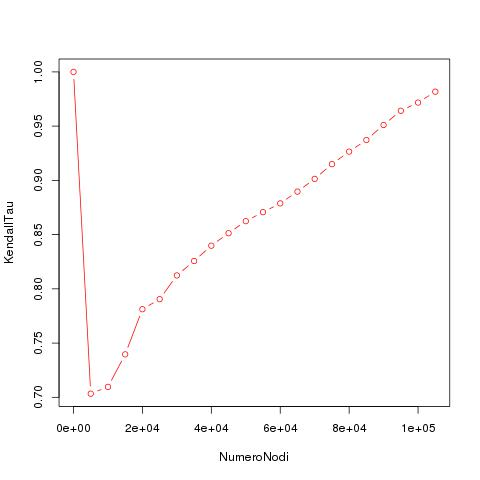
\includegraphics[height=9cm]{immagini/test1/trustranktestMode1_62}
 \caption{Test numero 1 (trustrank, 62). Calcolo della distanza dei vettori tra trustrank calcolato sull'intero grafo e trustrank calcolato sul grafo ricavato dai nodi visitati lungo una BFS partendo dal nodo 62.}
 \label{fig:test1trustModoB62}
\centering
 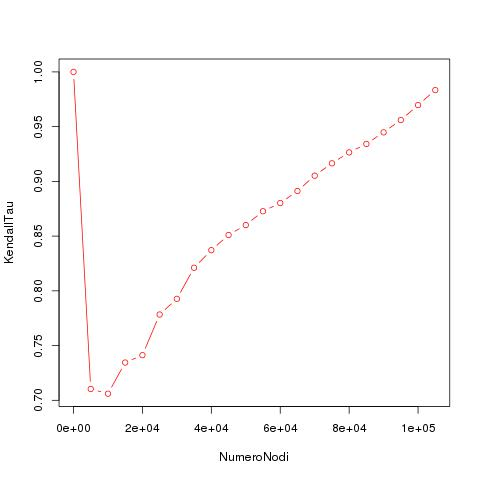
\includegraphics[height=9cm]{immagini/test1/trustranktestMode1_112}
 \caption{Test numero 1 (trustrank, 112). Calcolo della distanza dei vettori tra trustrank calcolato sull'intero grafo e trustrank calcolato sul grafo ricavato dai nodi visitati lungo una BFS partendo dal nodo 112.}
 \label{fig:test1trustModoB112}
\end{figure}

Eseguendo lo stesso test per valutare la distanza tra il vettore \(a\) di \textit{anti-trust rank} calcolato sull'intero grafo e il vettore \(\hat{a}_i\) calcolato sul grafo ottenuto dai nodi visitati durante una visita in ampiezza si nota che i risultati sono presocchè uguali ai precedenti due test. In particolare in figura \ref{fig:test1antitrustModoB62} è rappresentato il grafico della Tau di Kendal \(T_{a62}\) che mette a confronto il vettore \(a\) con il vettore \(\hat{a}_i\) dove la BFS ha come nodo sorgente 62 mentre in figura \ref{fig:test1antitrustModoB112} è rappresentato il grafico della Tau di Kendall \(T_{a112}\) che mette a confronto il vettore \(a\) con il vettore \(\hat{a}_i\) dove la BFS ha nodo sorgente 112; sull'asse delle ascisse è rappresentao il numero di nodi che sono visitati durante la BFS mentre sulle ordinate il corrispondente valore di Tau di Kendall tra il vettore di \(a\) calcolato sull'intero grafo e il vettore \(\hat{a}_i\) calcolato sul grafo ricavato dai nodi visitati attraverso una BFS a diversi passi, quindi \(i\) sarà uguale al numero dei nodi visitati ad un certo istante. Rispetto al test di \textit{trustrank} usando \textit{anti-trust rank} si nota che i grafici (senza considerare il primo valore per lo stesso motivo dei due test precedenti) hanno un andamento quasi logaritmico dove si ha come valore iniziale di Tau di Kendall 0.75 e come utlimi valori (stazionari) 0.95. Infatti un fattore evidente è che la Tau di Kendall tende a non superare il 0.95 per gli ultimi nodi incontrati nella BFS.

 \begin{figure}
\centering
 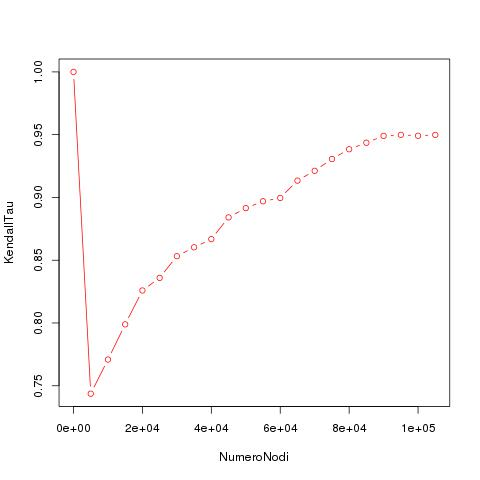
\includegraphics[height=9cm]{immagini/test1/antiTrustrankTestMode1_62}
 \caption{Test numero 1 (anti-trust rank, 62). Calcolo della distanza dei vettori tra anit-trust rank calcolato sull'intero grafo e anti-trust rank calcolato sul grafo ricavato dai nodi visitati lungo una BFS parteneo dal nodo 62.}
 \label{fig:test1antitrustModoB62}
\centering
 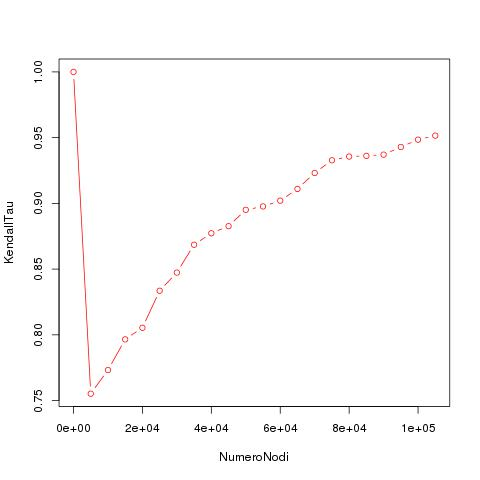
\includegraphics[height=9cm]{immagini/test1/antiTrustrankTestMode1_112}
 \caption{Test numero 1 (anti-trust rank, 112). Calcolo della distanza dei vettori tra anit-trust rank calcolato sull'intero grafo e anti-trust rank calcolato sul grafo ricavato dai nodi visitati lungo una BFS parteneo dal nodo 112.}
 \label{fig:test1antitrustModoB112}
\end{figure}

In figura \ref{fig:test1coplot62} sono riportati in un unico grafico i grafici rappresentati in figura \ref{fig:test1trustModoB62} relativo a \(T_{t62}\) e del  grafico \ref{fig:test1antitrustModoB62} relativo a \(T_{a62}\); in rosso è rappresentato il grafico raffigurante \(T_{t62}\) tra \textit{trustrank} calcolato sull'intero grafo e \textit{trustrank} calcolato sul grafo ottenuto dai nodi visitati a diversi passi di una BFS con nodo sorgente 62 mentre in verde è rappresentato il grafico  rappresentante \(T_{a62}\) tra \textit{anti-trust rank} calcolato sull'intero grafo e \textit{anti-trust rank} calcolato sul grafo ottenuto dai nodi visitati a diversi passi di una BFS con nodo sorgente 62. Quello che evince è che \(T_{a62}\) applicata al vettore \(a\) e \(\hat{a}_i\) cresce più velocemente rispetto a \(T_{t62}\) applicata a   \(t\) e \(\hat{t}_i\) ma che dopo la visita di circa 80000 \(T_{t62}\) assume valori più alti rispetto a \(T_{a62}\); infatti come avevamo detto i valori di \(T_{a62}\) tendono a fermarsi intorno a 0.95.\\
Tale comportamento tra \(T_{t62}\) e \(T_{a62}\) indica perciò che \textit{trustrank} eseguito online è più efficace di \textit{anti-trust rank} nel approssimare il loro comportamento offline ma solo dopo che sono stati visitati molti nodi mentre \textit{anti-trust rank} online riesce ad approssimare bene il suo comportamento anche se eseguito su un numero esiguo di nodi dell'intero grafo. Quindi  tra \textit{trustrank} e \textit{anti-trust rank} il miglior metodo per essere utilizzato in modalità online è \textit{anti-trust rank} perché tende ad approssimare fin da subito il comportamento offline anche avendo pochi nodi. Infatti il grafico in figura \ref{fig:test1coplot62} indica che \textit{anti-trust rank} eseguito durante la fase di crawling ritorna un vettore dove i valori tendono ad avvicinarsi rapidamente ai valore del vettore se \textit{anti-trust rank} fosse eseguito in modalità offline.\\
Le stesse valutazioni valgono tra il confronto dei due grafici in figura \ref{fig:test1trustModoB112} relativo a \(T_{t112}\) e \ref{fig:test1antitrustModoB112}  relativo a \(T_{a112}\) illustrato in figura \ref{fig:test1coplot112} dove in rosso è rappresentata la Tau di Kendall \(T_{t112}\) tra \textit{trustrank} calcolato sull'intero grafo e \textit{trustrank} calcolato sul grafo ottenuto dai nodi visitati a diversi passi di una BFS con nodo sorgente 112 mentre in verde è rappresentato il la Tau di Kendall \(T_{a112}\) tra \textit{anti-trust rank} calcolato sull'intero grafo e \textit{anti-trust rank} calcolato sul grafo ottenuto dai nodi visitati a diversi passi di una BFS con nodo sorgente 112. Come si nota anche in questo caso \textit{anti-trust rank} online riesce ad approssimare bene con  pochi nodi, rispetto al grafo completo, il comportamento offline differentemente a \textit{trustrank} che non riesce ad avere le stesse prestazioni tranne quando si hanno molti nodi (nel grafico in particolare piu di 80000) in questo caso le prestazioni di \textit{trustrank} superano quelle di \textit{anti-trust rnak}. Tali deduzioni si evincono dal fatto che \(T_{a112}\) cresce più rapidamente rispetto a \(T_{t112}\) ma dopo circa 80000 \(T_{a112}\) cresce più lentamente rispetto a \(T_{t112}\) che raggunge valori più alti.

 \begin{figure}
\centering
 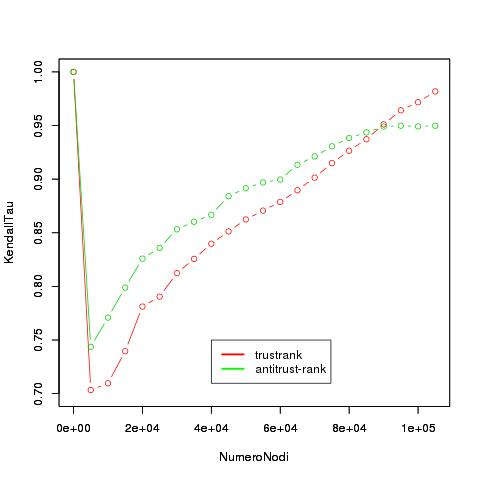
\includegraphics[height=9cm]{immagini/test1/coplotTrustAnti_62}
 \caption{Plotting del grafico \ref{fig:test1trustModoB62} e del  grafico \ref{fig:test1antitrustModoB62}}
 \label{fig:test1coplot62}
\centering
 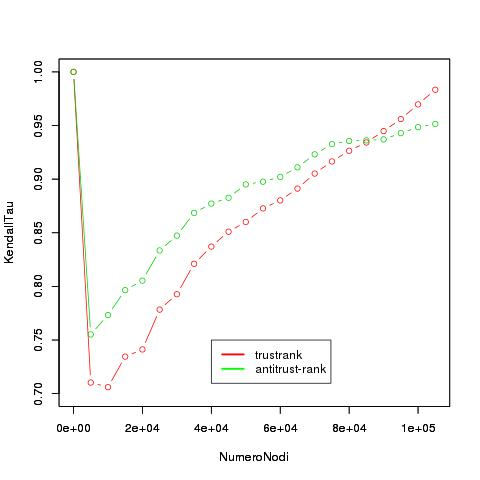
\includegraphics[height=9cm]{immagini/test1/coplotTrustAnti_112}
 \caption{Plotting del grafico \ref{fig:test1trustModoB112} e del  grafico \ref{fig:test1antitrustModoB112}}
 \label{fig:test1coplot112}
\end{figure}

\section{Test 2}
Il test consiste nel valutare la distanza tra due vettori, utilizzanto una Tau di Kendall \(T_t\), il vettore \(t\) di \textit{trustrank} calcolato sull'intero grafo e il vettore \(\hat{t}_i\) calcolato sul grafo ottentuto dai nodi visitati durante un visita in ampiezza; quindi la distanza viene calcolata ogni qual volta il numero di indici, del vettore \(\hat{t}_i\), a cui è possibile associare un valore aumenta  di un certo intervallo ovvero  quando la BFS visita un intervallo di nodi stabilito adentrandosi sempre di più nel grafo. Il test cosi descritto è simile al \textit{Test numero 1} ma differentemente del precedente in questo test nel determinare la distanza tra i due vettori si esaminano i soli indici dei vettori \(t\) e \(\hat{t}_i\) che fanno riferimento ai nodi etichettati come spam. Ugualmente il test viene effettuato per valutare \textit{anti-trust rank} ma in questo caso vengono confrontati, tramite la Tau di Kendall \(T_a\), i soli nodi indici dei due vettori \(a\) e \(\hat{a}_i\) che fanno riferimento a nodi etichettati come non spam.

Anche per questo test nella valutazione di \textit{trustrank} è stato usato come seedset l'insieme dei nodi etichettati non spam del dataset WEBSPAM-UK2007 mentre per \textit{anti-trustrank} è stato usto come seedset l'insieme dei nodi spam del dataset WEBSPAM-UK2007.

\begin{figure}
\centering
 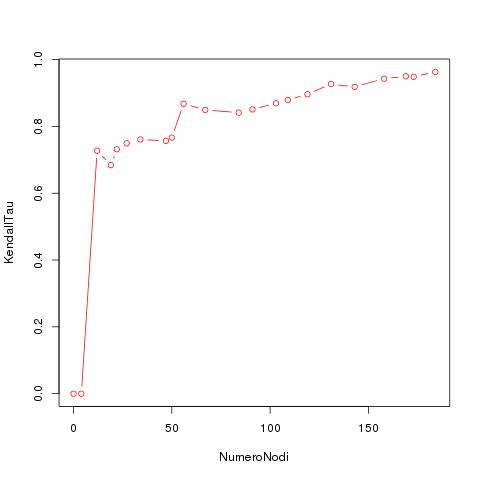
\includegraphics[height=9cm]{immagini/test2/trustrankBadNodesTestMode1_62}
 \caption{Test numero 2 (trustrank, 62). Calcolo della distanza dei vettori tra trustrank calcolato sull'intero grafo e trustrank calcolato sul grafo ricavato dai nodi visitati lungo una BFS partendo dal nodo 62 prendendo in considerazione i soli nodi spam. }
 \label{fig:test2trustModoB62}
\centering
 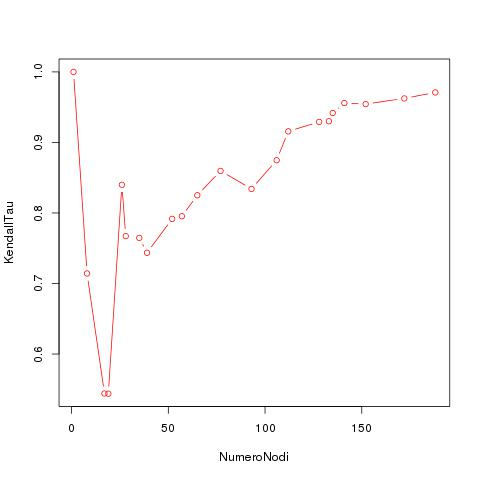
\includegraphics[height=9cm]{immagini/test2/trustrankBadNodesTestMode1_112}
 \caption{Test numero 2 (trustrank, 112). Calcolo della distanza dei vettori tra trustrank calcolato sull'intero grafo e trustrank calcolato sul grafo ricavato dai nodi visitati lungo una BFS partendo dal nodo 112 prendendo in considerazione i soli nodi spam.}
 \label{fig:test2trustModoB112}
\end{figure}

In figura \ref{fig:test2trustModoB62} è rappresentato il grafico della Tua di Kendall \(T_{t62}\) tra gli indici spam dei vettori \(t\) e \(\hat{t}_i\)  di tale dove il nodo sorgente della visita in ampiezza, con cui viene ricavato il grafo temporaneo sui cui viene calcolato \(\hat{t}_i\) è 62. Sull'asse delle ascisse è rappresentato il numero di nodi spam visitati durante la visita in ampiezza e sull'asse delle ordinate la Tau di Kendall \(T_{t62}\) calcolata a ogni intervallo di nodi visitati (compresi nodi spam e non spam).\\
Al primo passo, come per il \textit{test numero 1}, quando la visita in ampiezza ha visitato il solo nodo sorgente ci si aspetta che il vaore di \(T_{t62}\) sia  1 in quanto i vettori \(t\) e \(\hat{t}_i\) dovrebbero essere composti dal solo nodo visitato al primo passo (e quindi il nodo sorgente 62).  Ma dal momento che si stanno prendendo i soli nodi etichettati spam, il nodo 62 essendo etichettato non spam  viene scartato e quindi il vettore \(t\) e \(\hat{t}_i\) saranno vuoti e quindi \(T_{t62}\) al primo passo assume valore 0. Dopo di che con l'avanzanto della visita in ampiezza e appena questa incomincia ad incontrare nodi spam l'andamento del grafico cresce rapidamente fino a circa 0.7 per poi variare gradualemnte fino a circa 1.0.

\begin{figure}
\centering
 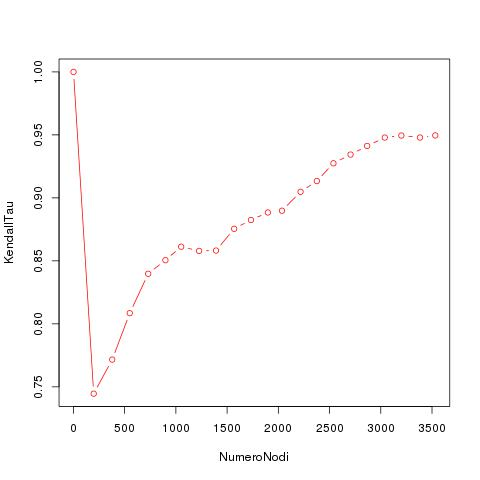
\includegraphics[height=9cm]{immagini/test2/antiTrustraktGoodNodesTestMode1_62}
 \caption{Test numero 2 (anti-trust rank, 62). Calcolo della distanza dei vettori tra anti-trust rank calcolato sull'intero grafo e anti-trust rank calcolato sul grafo ricavato dai nodi visitati lungo una BFS partendo dal nodo 62 prendendo in considerazione i soli nodi non spam. }
 \label{fig:test2antitrustModoB62}
\centering
 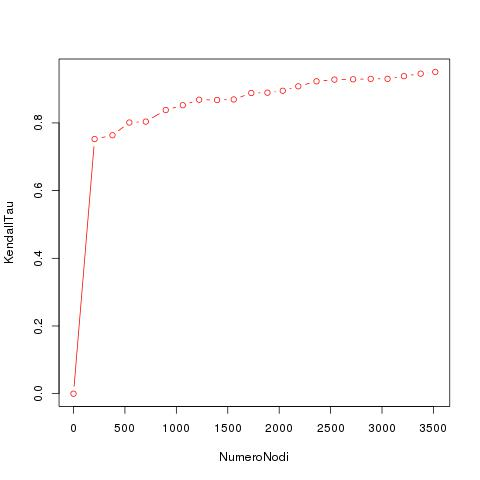
\includegraphics[height=9cm]{immagini/test2/antiTrustraktGoodNodesTestMode1_112}
 \caption{Test numero 2 (anti-trust rank, 62). Calcolo della distanza dei vettori tra anti-trust rank calcolato sull'intero grafo e anti-trust rank calcolato sul grafo ricavato dai nodi visitati lungo una BFS partendo dal nodo 112 prendendo in considerazione i soli nodi non spam. }
 \label{fig:test2antitrustModoB112}
\end{figure}

Il grafico della Tau di Kendall \(T_{t112}\)  calcolata  per ogni intervallo di nodi visitati tramite la visita in ampiezza con nodo sorgente 112 è rappresentato in figura \ref{fig:test2trustModoB112}.  Sull'asse delle ascisse è rappresentato il numero dei soli nodi spam visitati tramite la visita in ampiezza e sull'asse delle ordinate la Tau di Kendall \(T_{t112}\) calcolata a ogni intervallo di nodi visitati (compresi nodi spam e non spam).\\
In questo caso il primo valore della Tau di Kendall \(T_{t112}\) è 1 perché  il nodo sorgente 112 essendo spam verrà preso in considerazione nella valutazine, perciò i vettori \(t\) e \(\hat{t}_i\) saranno composti da un unico indice che fa riferimento al nodo 112 e la Tau di Kendall applicata a vettori composti da un solo elemento è uguale a 1. Ma con l'avanzamento della visita in ampiezza l'andamento della Tau di Kendall \(T_{t112}\) calcolata su \(t\) e \(\hat{t}_i\) varia tra circa 0.5 e 1.

Lo stesso test è stato applicato per valutare \textit{anti-trust rank}; in figura \ref{fig:test2antitrustModoB62} è illustrato il grafico relativo alla Tau di Kendall \(T_{a62}\) per il calcolo della distanza tra il vettore \(a\) e il vettore \(\hat{a}_i\) prendendo in considerazione i soli nodi non spam e la visita in ampiezza con nodo sorgente 62, mentre in figura \ref{fig:test2antitrustModoB112} è illustrato il grafico relativo alla Tau di Kendall \(T_{a112}\) per il calcolo della distanza tra il vettore \(a\) e il vettore \(\hat{a}_i\) prendendo in considerazione i soli nodi non spam e la visita in ampiezza con nodo sorgente 112. Sull'asse delle ascisse è rappresentato il numero dei soli nodi non spam incontrati tramite la visita in ampiezza tra tutti i nodi visitati e sull'asse delle ordinate la Tau di Kendall calcolato a ogni intervallo di nodi visitati.\\
Nel primo grafico si nota che a differenza del test su \textit{trustrank} con nodo sorgente, della BFS, 62 il primo valore della Tau di Kendall \(T_{a62}\), ovvero quando la visita in ampiezza ha visitato il solo nodo sorgente e quindi il grafo temporaneo è formato dal solo nodo 62, è 1 perchè in questo caso si esaminano i nodi non spam e tale nodo essendo non spam non viene rigettatto ma viene esaminato e quindi i vettori \(a\) e\(\hat{a}_i\) avranno un solo valore relativo al nodo 62 e perciò la Tau di Kendall \(T_{a112}\) al primo passo sarà 1. Con l'aumentare dei nodi visitati i valori di \(T_{a62}\) variano da circa 0.75 a 0.95.

Il secondo grafico mentre ha come primo valore della Tau di Kendall \(T_{a112}\) uguale a 0, questo perchè il grafo temporaneo è formato al primo passo èdal solo nodo 112 e quindi dal momento che 112 è un nodo spam viene rigettato e non esaminato. Perciò in questo caso sia il vettore \(a\) che il vettore \(\hat{a}_i\) avranno lunghezza zero fino al momento in cui la visita in ampiezza non incotra dei nodi non spam infatti nei passi successivi il grafico varia da circa 0.8 a circa 1.

\section{Test 3}
Questo test è stato ideato in modo da creare una situazione avversariale e mettere in difficoltà gli algoritmi di \textit{trustrank} e \textit{anti-trust rank} durante la loro esecuione in modalità online. Ovvero si è pensato di simulare il caso in cui il seedset che viene utilizzato dagli algoritmi (il quale va a definire la distribuzione di probabilità rappresentata dal vettore di preferenza dell'algoritmo di \textit{pagerank}) sia totalmente sbagliato e vedere i risultati che questo comporta nell'esecuzione in modalità online.

Il test, quindi, consiste (per la valutazione di \textit{trustrank}) nel eseguire una visita in ampiezza \(v_1\) da un nodo sorgente \(s\) e calcolare \textit{trustrank} sul grafo composto da tutti i nodi visitati alla fine della visita (che denomineremo \(t_v\)) dove il seedset \(S\) usato dall'algoritmo è composto dagli ultimi \(n\) nodi visitati da \(v_1\); dopodiché  si riesegue una seconda visita in ampiezza \(v_2\) con nodo sorgente \(s\) e si calcola \textit{trustrank}, per ogni intervallo di nodi visitati, sul grafo ottenuto da questi nodi (che denomineremo \(\hat{t}_i\)) con seedset \(S\) formato dagli ultimi \(n\) nodi visitati tramite la visita in ampiezza \(v_1\). Il numero di \(n\) nodi utilizzato è 3776 come la grandezza dell'insieme delle pagine eticchettate non spam nel dataset WEBSPAM-UK2007. Quindi si calcola la Tau di Kendall \(T_t\) tra il vettore \(t_v\) e il vettore \(\hat{t}_i\) ad ogni intervallo di nodi che vengono visitati tramite la visita in ampiezza \(v_2\).\\
Lo stesso test è stato applicato per valutare \textit{anti-trust rank}. In questo caso si esegue una visita in ampiezza \(v_1\) da un nodo sorgente \(s\) e viene calcolato \textit{anti-trust rank} sul grafo composto da tutti i nodi visitati alla fine della visita (denominato \(a_v\)) e il seedset \(S\) utilizzato per il calcolo di \(a_v\) è composto dagli ultimi \(n\) nodi visitati da \(v_1\); successivamente si riesegue una seconda visita in ampiezza \(v_2\) con nodo sorgente \(s\) e si calcola \textit{anti-trust rank}, per ogni intervallo di nodi visitati, sul grafo ottenuto da questi nodi (che denomineremo \(\hat{a}_i\)) dove il seedset usato dall'algoritmo di \textit{anti-trust rank} è formato come prima dai nodi dell'insieme \(S\). Infine  viene calcolata la Tau di Kendall \(T_t\) tra il vettore \(a_v\) e il vettore \(\hat{a}_i\) ogni intervallo di nodi che vengono visitati tramite la visita in ampiezza. Anche in questo caso il numero di nodi \(n\) scelti come seedset sarà 3776.\\
Durante il calcolo di \(\hat{t}_i\) e di \(\hat{a}_i\), sul grafo temporaneo ottenuto dai nodi lungo la visita in ampiezza \(v_2\), finché la visita non incontrerà i nodi facenti parte dell'insieme \(S\) il vettore di preferenza con cui si calcolerà \(\hat{t}_i\) e \(\hat{a}_i\) sarà una distribuzione uniforme, il che siginifica che nel caso di \textit{trustrank} sarà come calcolare \textit{pagerank} mentre nel caso di \textit{anti-trustrank} sarà come calcolare \textit{pagerank} trasposto. Nel momento in cui la visita in ampiezza incomincerà ad incotrare qualche nodo dell'insieme \(S\) allora il vettore di preferenza verrà manipolato con una distribuzione personalizzata basata sui nodi appartenenti all'insieme \(S\) che sono stati visitati. 


In figura \ref{fig:test3coplotTrustAntiModeB62} è rappresentato il grafico del test eseguito per valutare \textit{trustrank} e \textit{anti-trust rank}; in particolare è raffigurata la Tau di Kendall \(T_{t62}\) tra il vettore \(t_v\) e il vettore \(\hat{t}_i\) calocolato sul grafo temporaneo ricavato dalla visita in ampiezza \(v_2\) con nodo sorgetne 62, e la Tau di Kendall \(T_{a62}\) tra il vettore \(a_v\) e il vettore \(\hat{a}_i\) calocolato sul grafo temporaneo ricavato dalla visita in ampiezza \(v_2\) con nodo sorgente 62. Sull'asse delle ascisse è rappresentato il numero di nodi visitati tramite la visita \(v_2\) mentre sull'asse delle ordinate il valore delle Tau di Kendall \(T_{t62}\) e \(T_{a112}\). In rosso è illustrato il grafico della Tau di Kendall \(T_{t62}\)  mentre in verde è rappresentato l'andamento della Tau di Kendall \(T_{a62}\). La Tau di Kendall \(T_{t62}\) e della Tau di Kendal \(T_{a62}\) dove \(T_{a62}\) cresce rapidamente rispetto alla Tau di Kendall \(T_{t62}\) che cresce lentamente ma tale comportamento cambia dopo che \(v_2\) ha incontrato circa 80000 nodi. 
\begin{figure}
\centering
 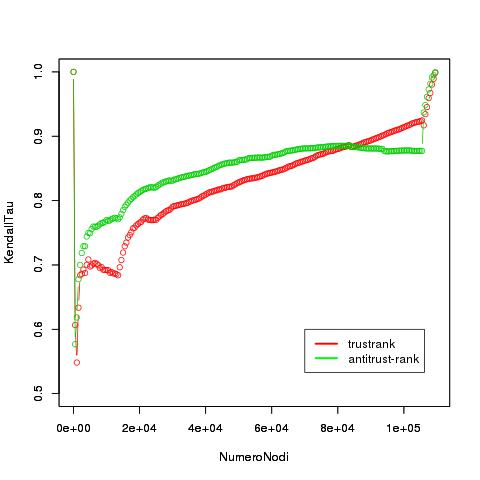
\includegraphics[height=9cm]{immagini/test3/coplotTrustAnti_Mode1_set3776_62}
 \caption{Test numero 3 . In rosso, calcolo della Tau di Kendall, nel Modo\_B, tra il vettore $t_v$ e il vettore $\hat{t}_i$ per ogni intervallo di nodi visitati della BFS partendo dal nodo 62. In verde calcolo della Tau di Kendall, nel Modo\_B, tra il vettore $a_v$ e il vettore $\hat{a}_i$ per ogni intervallo di nodi visitati della BFS partendo dal nodo 62}
 \label{fig:test3coplotTrustAntiModeB62}
\centering
 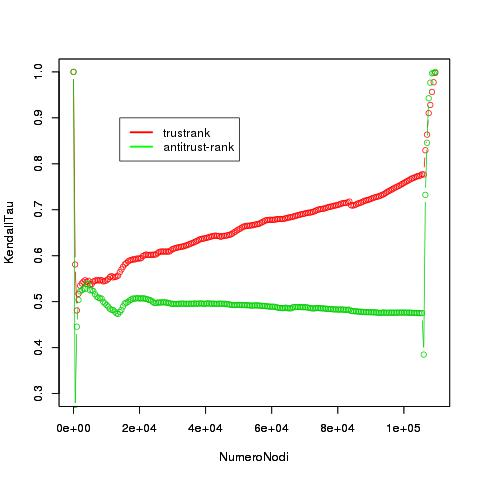
\includegraphics[height=9cm]{immagini/test3/coplotTrustAnti_Mode1_set3776_62_alpha0005}
  \caption{Test numero 3 . In rosso, calcolo della Tau di Kendall, nel Modo\_B, tra il vettore $t_v$ e il vettore $\hat{t}_i$, dove $\alpha$ è impostato a 0.005, per ogni intervallo di nodi visitati della BFS partendo dal nodo 62. In verde calcolo della Tau di Kendall, nel Modo\_B, tra il vettore $a_v$ e il vettore $\hat{a}_i$, dove $\alpha$ è impostato a 0.005, per ogni intervallo di nodi visitati della BFS partendo dal nodo 62}
 \label{fig:test3coplotTrustAntiModeB620005}
\end{figure}

 

 
